\begin{figure*}[t]
    \makebox[\textwidth][c]{
    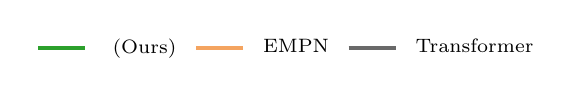
\begin{tikzpicture}
    \tikzstyle{every node}=[font=\scriptsize]
    \definecolor{tabblue}{RGB}{31, 119, 180}
\definecolor{taborange}{RGB}{255, 127, 14}
\definecolor{tabgreen}{RGB}{44, 160, 44}
\definecolor{tabred}{RGB}{214, 39, 40}
\definecolor{tabpurple}{RGB}{148, 103, 189}
\definecolor{tabbrown}{RGB}{140, 86, 75}
\definecolor{tabpink}{RGB}{227, 119, 194}
\definecolor{tabgray}{RGB}{127, 127, 127}
\definecolor{tabolive}{RGB}{188, 189, 34}
\definecolor{tabcyan}{RGB}{23, 190, 207}
\definecolor{lightblue}{RGB}{173, 216, 230}
\definecolor{sandybrown}{RGB}{244, 164, 96}
\definecolor{darkgrey}{RGB}{169, 169, 169}
\definecolor{dimgrey}{RGB}{105, 105, 105}
\definecolor{olivedrab}{RGB}{107, 142, 35}
\definecolor{darkviolet}{RGB}{148, 0, 211}
\definecolor{darkgoldenrod}{RGB}{184, 134, 11}
\definecolor{darkblue}{RGB}{0, 0, 139}
\definecolor{orchid}{RGB}{218, 112, 214}

    \begin{axis}[%
        hide axis,
        xmin=10,
        xmax=50,
        ymin=0,
        ymax=0.1,
        legend style={
            draw=white!15!black,
            legend cell align=left,
            legend columns=3,
            legend style={
                draw=none,
                column sep=1ex,
                line width=1pt,
            }
        },
        ]
        \addlegendimage{line legend, tabgreen, ultra thick} % Thicker line here
        \addlegendentry{\textbf{\model} (Ours)}
        \addlegendimage{line legend, sandybrown, ultra thick} % Thicker line here
        \addlegendentry{EMPN}
        \addlegendimage{line legend, dimgrey, ultra thick} % Thicker line here
        \addlegendentry{Transformer}
    \end{axis}
\end{tikzpicture}

    }
    \centering
    \begin{subfigure}[b]{0.25\linewidth}
        \includegraphics[width=\textwidth]{ICLR_2025/Figures/eval_all_6_tasks/smooth_consistent_eval_Isaac-Rigid-Sliding-Multi-v0_eval_all.pdf}
    \end{subfigure}%
    \begin{subfigure}[b]{0.25\linewidth}
    \includegraphics[width=\textwidth]{ICLR_2025/Figures/eval_all_6_tasks/smooth_eval_Isaac-Rigid-Insertion-Multi-v0_eval_consistent.pdf}
    \end{subfigure}%
    %\hfill
    \begin{subfigure}[b]{0.25\linewidth}
        \includegraphics[width=\textwidth]{ICLR_2025/Figures/eval_all_6_tasks/smooth_eval_Isaac-Rigid-Insertion-Multi-Two-Actuators-v0_eval_consistent.pdf}
    \end{subfigure}%
    %\hfill
    \begin{subfigure}[b]{0.25\linewidth}
        \includegraphics[width=\textwidth]{ICLR_2025/Figures/eval_all_6_tasks/eval_30_Isaac-Rigid-Pushing-No-Contact-Multi-v0_eval_all.pdf}
    \end{subfigure}
        
    \begin{subfigure}[b]{0.25\linewidth}
        \includegraphics[width=\textwidth]{ICLR_2025/Figures/eval_all_6_tasks/smooth_eval_Isaac-Rope-Closing-v0_eval_all.pdf}
    \end{subfigure}
    %\hfill
    \begin{subfigure}[b]{0.25\linewidth}
        \includegraphics[width=\textwidth]{ICLR_2025/Figures/eval_all_6_tasks/smooth_eval_Isaac-Rope-Shaping-v0_eval_all.pdf}
    \end{subfigure}
    %\hfill
    \begin{subfigure}[b]{0.25\linewidth}
        \includegraphics[width=\textwidth]{ICLR_2025/Figures/eval_all_6_tasks/smooth_eval_Isaac-Cloth-Hanging-Multi-v0_eval_all.pdf}
    \end{subfigure}
    
    \caption{\update{Evaluation} curves for our \rebuttal{seven} manipulation tasks, comparing HEPi (ours), EMPN, and Transformer baselines. Results are averaged over 10 seeds, using IQM with 95\% confidence intervals. HEPi consistently outperforms EMPN and Transformer in tasks requiring complex exploration and heterogeneity handling, such as \textit{rigid-insertion-two-agents-3D}, \rebuttal{\textit{rigid-pushing-2D}} and \textit{cloth-hanging-3D}.}
    \vspace{-0.2cm}
    \label{fig:results_main_6_tasks}
\end{figure*}